\documentclass[12pt,a4paper]{article}
\usepackage[utf8]{inputenc}
\usepackage{amsmath}
\usepackage{amsfonts}
\usepackage{amssymb}


\usepackage{cmap} % для кодировки шрифтов в pdf
\usepackage[T1]{fontenc}
\usepackage{hhline}
\usepackage[unicode]{hyperref}
\usepackage{multirow}
\usepackage{array}
\usepackage{amsmath}
\usepackage{bm}
\usepackage{textcomp}
\usepackage[russian]{babel}
\usepackage{graphicx} % для вставки картинок
\usepackage{amssymb,amsfonts,amsmath,amsthm} % математические дополнения от АМС
\usepackage{indentfirst} % отделять первую строку раздела абзацным отступом тоже
% Поля
\usepackage{geometry}
\geometry{left=2cm}
\geometry{right=1.5cm}
\geometry{top=2.4cm}
\geometry{bottom=2.cm}

%%%%%%%%%%%%%%%%%%%%%%%%%%%%%%%     

\linespread{1.5} % полуторный интервал
\frenchspacing




\begin{document}
	
	\begin{titlepage}
		
		\begin{center}
			\begin{large}
				Санкт-Петербургский Политехнический университет\\ Петра Великого\\
				Институт прикладной математики и механики\\
			\end{large}
			\vspace{0.2cm}
			Высшая школа прикладной математики и вычислительной физики\\
			
		\end{center}
		
		\vspace{3cm}
		\begin{center}
			\textbf{Отчёт\\ по лабораторной работе №1\\ по дисциплине\\ "математическая статистика"}
		\end{center}
		
		\vspace{3cm}
		
		\vbox{%
			\hfill%
			\vbox{%
				\hbox{Выполнил студент:}%
				\hbox{\break}
				\hbox{Аникин Алксандр Алксеевич,}%
				\hbox{группа 3630102$\backslash$80201}%
				\hbox{\break}
				\hbox{\break}
				\hbox{Проверил:}
				\hbox{\break}
				\hbox{к.ф.-м.н., доцент}
				\hbox{Баженов Александр Николаевич}
			}%
		} 
		\vfill
		
		\begin{center}
			Санкт-Петербург, 2021
		\end{center}
		
	\end{titlepage}
	\tableofcontents
	\newpage
	
	\listoffigures
	\newpage
	
	\section{Постановка задачи}
	Для следующих распределений:
	\begin{itemize}
		\item Нормальное распределение $\textit{N}(\textit{x}, 0, 1)$
		\item Распределение Коши $\textit{C}(\textit{x}, 0, 1)$
		\item Распределение Лапласа $\textit{L}(\textit{x}, 0, \frac{1}{\sqrt{2}})$
		\item Распределение Пуассона $\textit{P}(\textit{k}, 10)$
		\item Равномерное распределение $\textit{U}(\textit{x}, -\sqrt{3}, \sqrt{3})$
	\end{itemize}
	Сгенерировать выборки размером 10, 50 и 1000 элементов. Построить на одном рисунке гистограмму и график плотности распределения.
	\newpage
	
	\section{Теория}
	
	\subsection{Рассматриваемые распределения}
	Плотности:
	\begin{itemize}
		\item Нормальное распределение:
		\begin{equation}\label{norm}
		\textit{N}(\textit{x}, 0, 1)=\frac{1}{\sqrt{2\pi}}e^{-\frac{x^2}{2}}
		\end{equation}
		
		\item Распределение Коши:
		\begin{equation}\label{cauchy}
		\textit{C}(\textit{x}, 0, 1)=\frac{1}{\pi}\frac{1}{x^2+1}
		\end{equation}
		
		\item Распределение Лапласа:
		\begin{equation}\label{laplace}
		\textit{L}(\textit{x}, 0, \frac{1}{\sqrt{2}})=\frac{1}{\sqrt{2}}e^{-\sqrt{2}|x|}
		\end{equation}
		
		\item Распределение Пуассона:
		\begin{equation}\label{poisson}
		\textit{P}(\textit{k}, 10)=\frac{10^k}{k!}e^{-10}
		\end{equation}
		
		\item Равномерное распределение:
		\begin{equation}\label{uniform}
		\textit{U}(\textit{x}, -\sqrt{3}, \sqrt{3})=
		\left\{
		\begin{array}{l}
		\frac{1}{2\sqrt{3}} \quad \text{при} \quad |x|\leq \sqrt{3}\\
		0 \quad \quad \text{при} \quad |x|>3
		\end{array}
		\right.
		\end{equation}
	\end{itemize}
	\subsection{Гистограмма}
	\subsubsection{Построение гистограммы}
	Множество значений, которое может принимать элемент выборки, разбивается на несколько интервалов. Чаще всего эти интервалы берут одинаковыми, но это не является строгим требованием. Эти интервалы откладываются на горизонтальной оси, затем над каждым рисуется прямоугольник. Если все интервалы были одинаковыми, то высота каждого пря моугольника пропорциональна числу элементов выборки, попадающих в соответствующий интервал. Если интервалы разные, то высота прямоугольника выбирается таким образом, чтобы его площадь была пропорциональна числу элементов выборки, которые попали в этот интервал \cite{hist_ref}.
	\newpage
	
	\section{Реализация}
	Лабораторная работа выполнена на языке Python 3.8 с помощью загружаемых пакетов SciPy и MatPlotLib. Исходный код лабораторной работы находится на GitLab репозитории.
	\newpage
	
	\section{Результаты}
	\subsection{Гистограмма и график плотности распределения}
	
	\centering{
		\begin{figure}[h!]
			\begin{minipage}[h]{0.3\linewidth}
				\centering{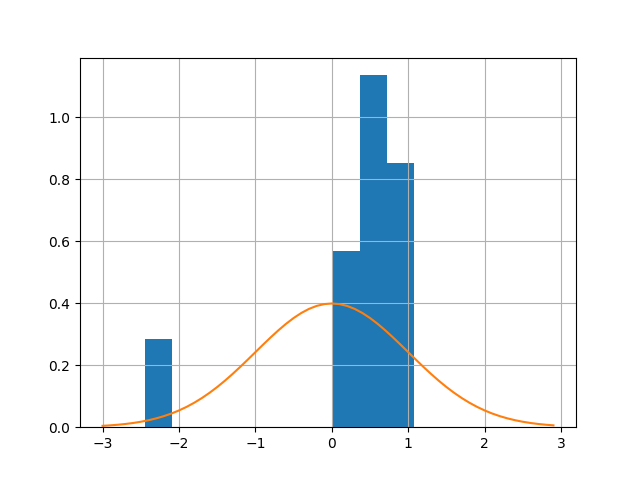
\includegraphics[width=1.25\linewidth]{../plots/normal10.png}\\\centering{$n=10$}}
			\end{minipage}
			\hfill
			\begin{minipage}[h]{0.3\linewidth}
				\centering{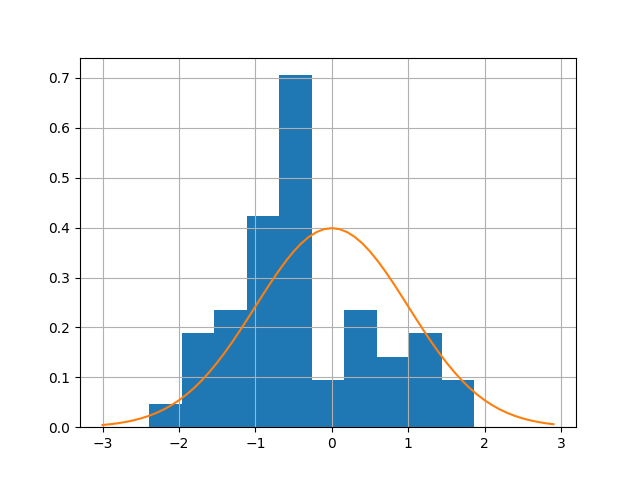
\includegraphics[width=1.25\linewidth]{../plots/normal50.png}\\\centering{$n=50$}}
			\end{minipage}
			\hfill
			\begin{minipage}[h]{0.3\linewidth}
				\centering{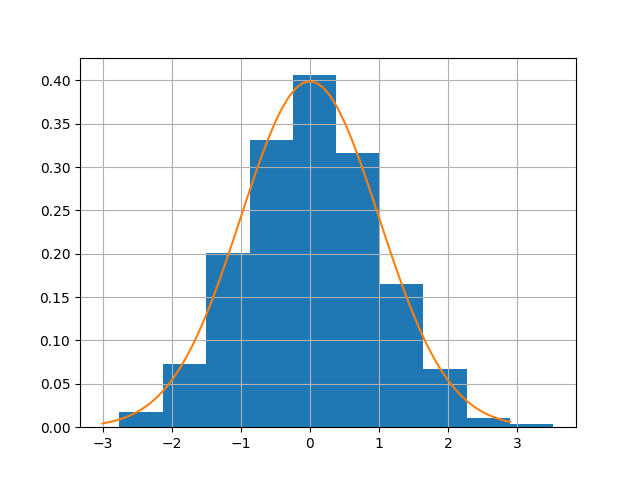
\includegraphics[width=1.25\linewidth]{../plots/normal1000.png}\\\centering{$n=1000$}}
			\end{minipage}
			\caption{Нормальное распределение (\ref{norm}), гистограмма и график функции плотности}
			\label{ris:normal}
		\end{figure}
	}
	
	\begin{figure}[h!]
		\begin{minipage}[h]{0.3\linewidth}
			\centering{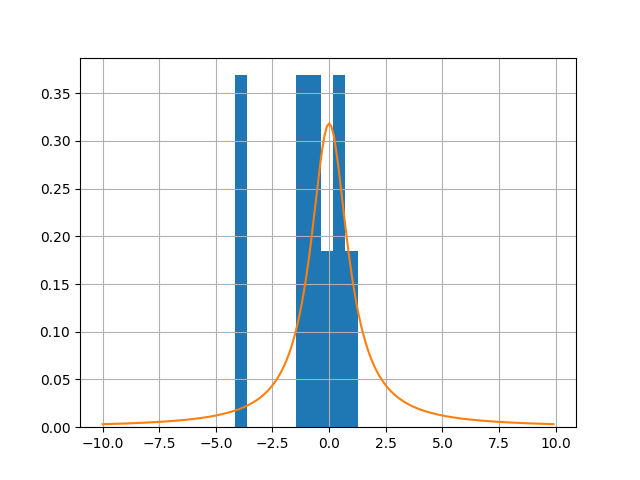
\includegraphics[width=1.25\linewidth]{../plots/cauchy10.png}\\\centering{$n=10$}}
		\end{minipage}
		\hfill
		\begin{minipage}[h]{0.3\linewidth}
			\centering{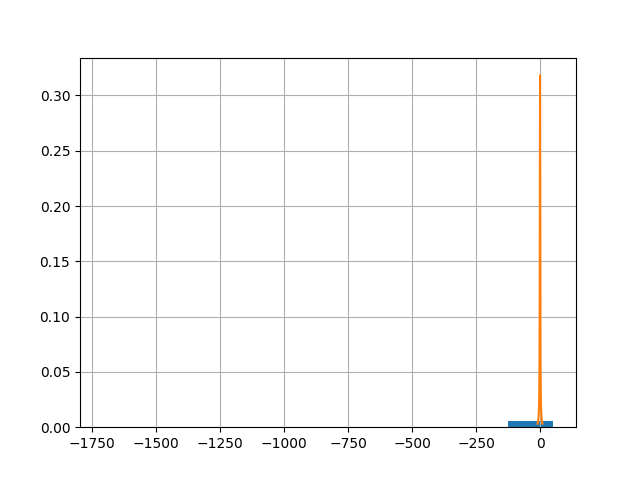
\includegraphics[width=1.25\linewidth]{../plots/cauchy50.png}\\\centering{$n=50$}}
		\end{minipage}
		\hfill
		\begin{minipage}[h]{0.3\linewidth}
			\centering{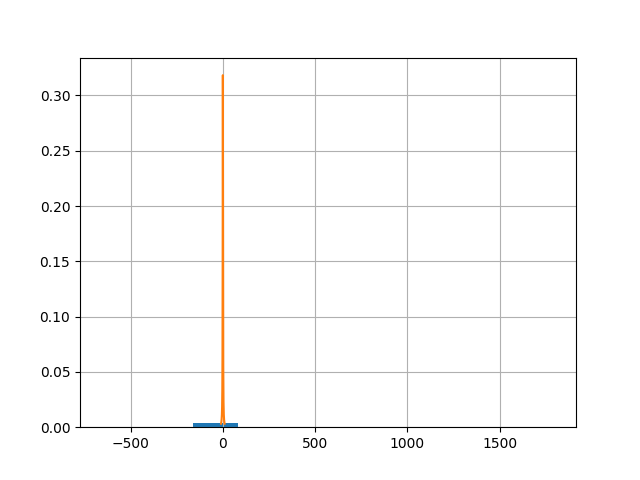
\includegraphics[width=1.25\linewidth]{../plots/cauchy1000.png}\\\centering{$n=1000$}}
		\end{minipage}
		\caption{Распределение Коши (\ref{cauchy}), гистограмма и график функции плотности}
		\label{ris:cauchy}
	\end{figure}
	
	\begin{figure}[h!]
		\begin{minipage}[h]{0.3\linewidth}
			\centering{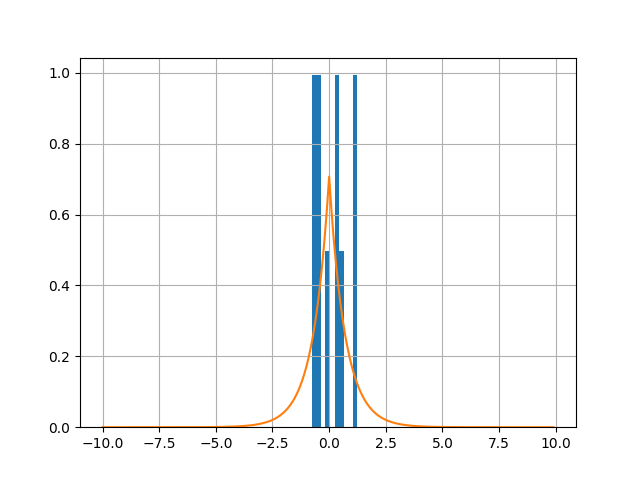
\includegraphics[width=1.25\linewidth]{../plots/laplace10.png}\\\centering{$n=10$}}
		\end{minipage}
		\hfill
		\begin{minipage}[h]{0.3\linewidth}
			\centering{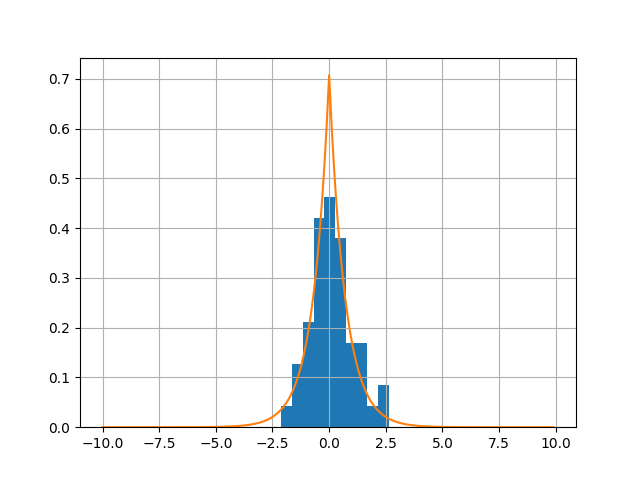
\includegraphics[width=1.25\linewidth]{../plots/laplace50.png}\\\centering{$n=50$}}
		\end{minipage}
		\hfill
		\begin{minipage}[h]{0.3\linewidth}
			\centering{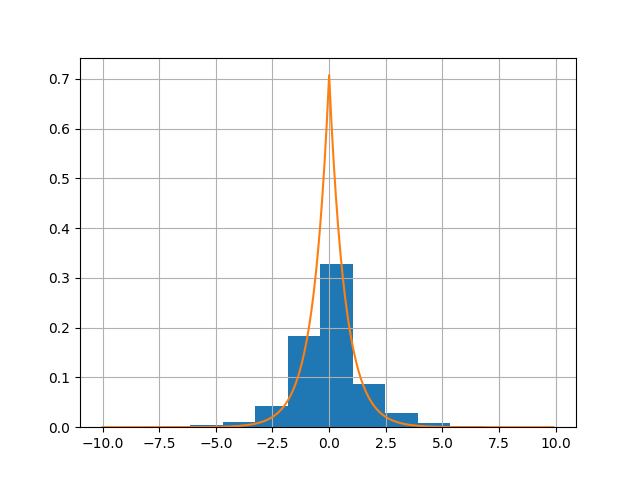
\includegraphics[width=1.25\linewidth]{../plots/laplace1000.png}\\\centering{$n=1000$}}
		\end{minipage}
		\caption{Распределение Лапласа (\ref{laplace}), гистограмма и график функции плотности}
		\label{ris:laplace}
	\end{figure}
	
	\begin{figure}[h!]
		\begin{minipage}[h]{0.3\linewidth}
			\centering{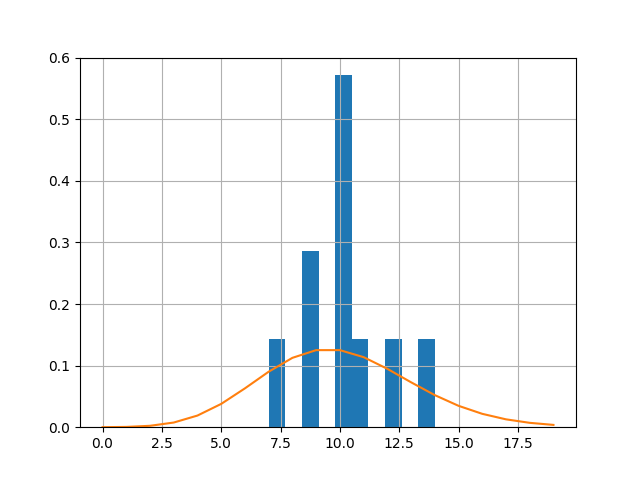
\includegraphics[width=1.25\linewidth]{../plots/poisson10.png}\\\centering{$n=10$}}
		\end{minipage}
		\hfill
		\begin{minipage}[h]{0.3\linewidth}
			\centering{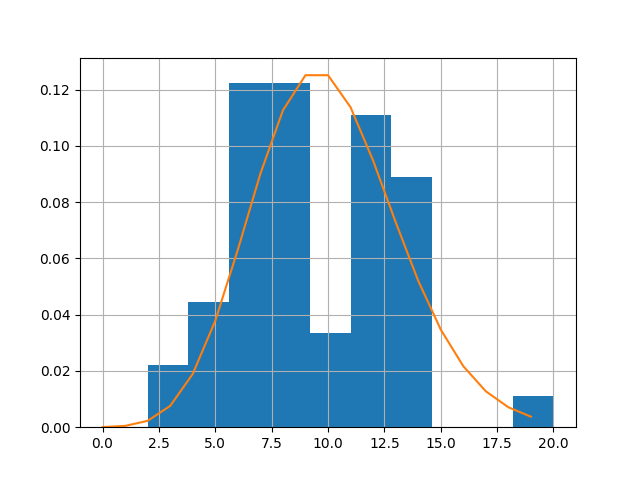
\includegraphics[width=1.25\linewidth]{../plots/poisson50.png}\\\centering{$n=50$}}
		\end{minipage}
		\hfill
		\begin{minipage}[h]{0.3\linewidth}
			\centering{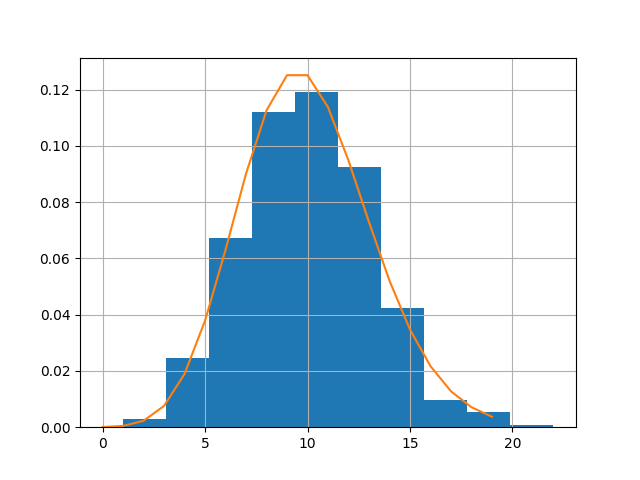
\includegraphics[width=1.25\linewidth]{../plots/poisson1000.png}\\\centering{$n=1000$}}
		\end{minipage}
		\caption{Распределение Пуассона (\ref{poisson}), гистограмма и график функции плотности}
		\label{ris:poisson}
	\end{figure}
	\newpage
	\begin{figure}[h!]
		\begin{minipage}[h]{0.3\linewidth}
			\centering{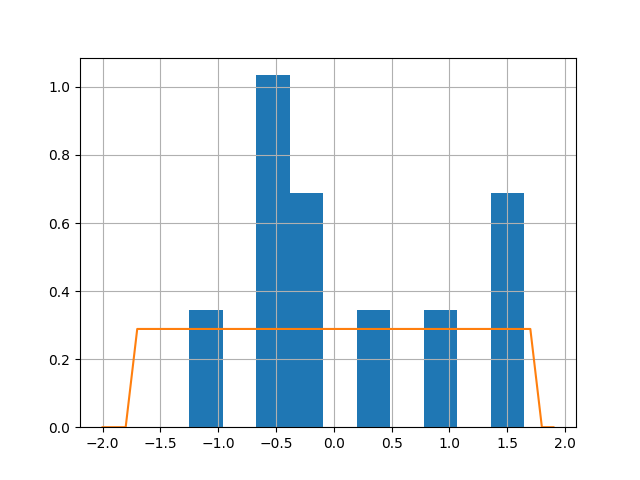
\includegraphics[width=1.25\linewidth]{../plots/uniform10.png}\\\centering{$n=10$}}
		\end{minipage}
		\hfill
		\begin{minipage}[h]{0.3\linewidth}
			\centering{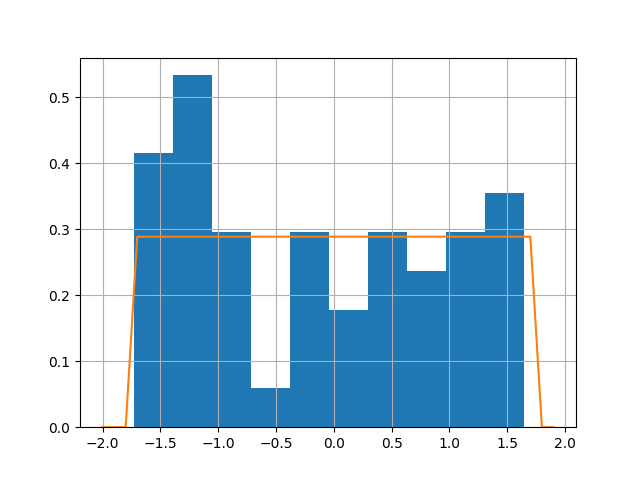
\includegraphics[width=1.25\linewidth]{../plots/uniform50.png}\\\centering{$n=50$}}
		\end{minipage}
		\hfill
		\begin{minipage}[h]{0.3\linewidth}
			\centering{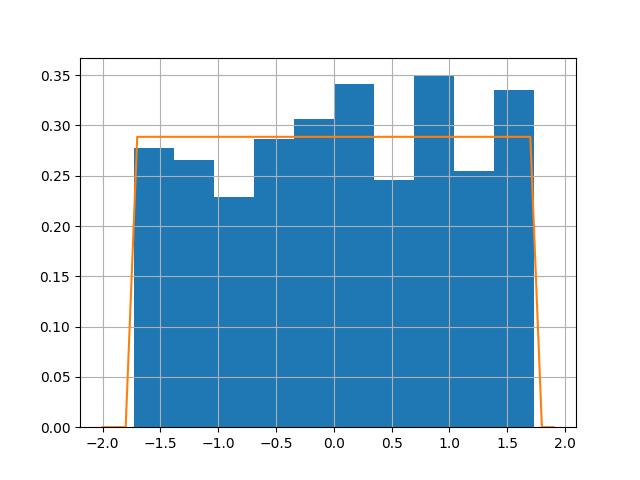
\includegraphics[width=1.25\linewidth]{../plots/uniform1000.png}\\\centering{$n=1000$}}
		\end{minipage}
		\caption{Равномерное распределение (\ref{uniform}), гистограмма и график функции плотности}
		\label{ris:uniform}
	\end{figure}
	\clearpage
	\newpage
	
	\begin{flushleft}
		\begin{thebibliography}{1}
			\addcontentsline{toc}{section}{\bibname}
			\bibitem{hist_ref}  Histogram. URL: \url{https://en.wikipedia.org/wiki/Histogram}
		\end{thebibliography}
	\end{flushleft}
	
	
\end{document}